% !TEX root = /Users/royc/Google_Drive/Thesis/RoyC_Umass_Thesis.tex
\chapter{Discussion} 
\label{Disc}
\lhead{Chapter 5. \emph{Discussion}} 
%----------------------------------------------------------------------------------------
\section{Concerning the Transcriptome}
  \label{Disc:sec:Future of Dynamic long RNAs}

  Deep sequencing of transcriptomes has revolutionized biology. Previously, transcript identification and characterization involved significant labor, cost, and materials. In the mid-90's, microarray technology \citep{Schena1995a} gave a tantalizing glimpse into how genes were expressed, but were limited to probed, and therefore known, sequences. Yet, the green and red landscapes hinted at incredible complexity. Full realization of this complexity would have to wait for technology to catch up.

  RNA-seq is possible due to incremental improvements in numerous supportive technologies included: (1) digital optics; (2) microscopy; (3) slide chemistry; (4) colony PCR; and (4) nucleic-acid alignment. A HiSeq 2500 relies on all of these technologies (and others) to produce the >100,000,000 sequences that allow scientists to peer into the transcriptional output of a genome.

  Biologists can now think beyond mRNAs and small RNAs. The former captured our interest for 30+ years \citep{Furuichi1975,Wei1975}, while the later has been on a run-away train since 1998 \citep{Fire1998}. Now included on the list of captivating RNAs are Long non-coding RNAs (lncRNAs). All classes of RNA are now routinely measured by HTS. However, many biologically-trained and minded scientists find themselves overwhelmed by methods and approaches used to tackle these biological ``big data.'' Current training programs do not provide most with required skills in statistics, programing, and experimental design necessary to work with genome-wide data (see section \ref{Disc:subsec:Biologists need Comp Skills}). The richness of these data often results in unasked---and unanswered---testable hypothesis, answers to which are just sitting in public data repositories \citep{Plocik2013}.

  This discussion will focus on \textit{long} RNA class that contain traditional mRNA features---a 5\textprime~m7G Cap, ligated exons, and a poly(A)+ tail. Many of these long mRNAs are extremely dynamic. So much so that until HTS and RNA-Seq, comprehensive investigation of their complexity was impossible.

  \subsection{Pervasive transcription}
    \label{Disc:subsec:Pervasive Tx}

    There are 2,598,960 different Poker hands possible from a 52-card deck. There are 1,098,240 different single-pair combinations, with a probability of obtaining one being almost 50\%. Compare this to a ``Royal Flush'', for which there are only 4 options, and a probability of 649,739:1 or 1.54 * 10$^{-6}$! It is these numbers that makes it possible to play Poker for hours on end. 

    Biology uses similar combinatorics to arrange exons into unique and rare combinations. This is especially true complex eukaryotic organisms, where virtually all genes are alternatively spliced (Figure \ref{Intro:fig:numGenesAndNumSpliced}). Accurate determination and assembly of each card (exon) that comprises a hand (transcript) is a major ``known unknown'' \citep{Rumsfeld2011} of research into long RNAs.

    The ENCODE papers of late 2012 suggest that 95\% of the genome is functional \citep{Dunham2012}, a heavily debated finding \citep{Graur2013,Bhattacharjee2014}. \citet{Djebali2012} focused on transcription in the ENCODE cell lines (discussed in section \ref{Intro:subsec:IsoformsPerGene}) and concluded that 75\% of the genome is transcribed into RNA. Additionally, ``GENCODEv7'' includes 9,640 manually curated lncRNA loci. These lncRNA are some of the most novel and functionally interesting class of long RNAs \citep{Derrien2012,Pauli2011}. While ENCODE was performed using multiple human cancerous cell lines, these results do support the ability of HTS to reveal transcriptional diversity.

  \subsection{A Need for Transcript Assembly}
    \label{Disc:subsec:need for Tx assembly}

    The field of transcriptome assembly is in its infancy (see section \ref{Intro:subsec:Tx Assembly}). Current transcript assembly algorithms only provide predictions and probabilities for the existence of real molecules. Until RNA is directly and completely sequenced from single cells or molecular compartments, researchers will always be forced to make compromises in annotation and quantification \citep{Ozsolak2010,Steijger2013}. Once technology advances to the point where a transcriptome is as accurately and quickly determined as a genome, exciting research into the subtle and nuanced complexity of transcriptome regulation will be revealed (e.g. what makes one twin \textit{molecularly} different from another?).

    What is required to improve our ability to quickly and accurately assemble transcriptomes? Simulations indicate that improvements will not come from longer read lengths \citep{Chang2014c}. These simulations also demonstrate that the accuracy of current \textit{de novo} (see section \ref{Intro:subsec:Tx Assembly}) assemblers decreases sharply with increased increase alternative splicing within the transcriptome. Systemic assessment of RNA-Seq transcript reconstruction methods have concluded what is likely to be the most revolutionary step toward accurate transcriptome assembly---single pass sequencing of single transcripts \citep{Engstrom2013,Steijger2013}. Results presented by \citep{Sharon2013}, demonstrating inherent constraints imposed by requiring RT to convert long RNAs to long cDNAs, mean that this future single-molecule sequencing will have to be of the RNA directly. This will be especially important and informative to measure RNA modifications such as N6-methyl-adenosine \citep{Pan2013}

  \subsection{Tissue and Cell Specificity}
    \label{Disc:subsec:Tissue-specific Tx expression}

    As discussed in section \ref{Intro:subsec:Alternative Splicing}, mechanisms of alternative splicing are frequently tissue-, time-, and cell- specific. Landmark studies examining alternative splicing in different organ systems, from evolutionarily-distant organims, found that alternative splicing is more comparable between organs of different animals than between different organs from the \textit{same} animal \citep{Barbosa-Morais2012,Merkin2012}. \citet{Brown2014} analyzed the \flies{} transcriptome, and observed that alternative splicing could be better described as ``tissue-specific splicing''. Further, tissue-specific lncRNA expression has been recently reported \citep{Washietl2014}, adding to the importance of sample resolution when performing transcriptome analysis.

    The concept of ``tissue-specific splicing'' brings up a subtle but important consideration concerning alternative splicing research. The concept of alternative splicing conjures an image of dynamic post-transcription RNA processing, allowing cells to quickly respond changes in environment, programming, or stimuli. Yet, as demonstrated by the studies just mentioned, most alternative splicing is not that dynamic. In fact, the main reason many of these events are even considered \textit{alternative} is because we are comparing transcriptomes of different tissues. Is that a fair comparison?

    By the current definition these events are indeed \textit{alternative}, but significance does that label carry? The label of alternative communicates that RNA products of a gene can be processed in multiple ways, but if they are typically \textit{not}, does this capability matter when HTS allows analysis of very specific biological samples and time points? These questions underscore the importance of advances in transcriptme assembly keeping step with advancements in HTS technology and ever-increasing sample resolution.

\section{In the haystack: piRNA Precursors}
  \label{Disc:sec:piRNA precursors}

  Chapter \ref{MolCel} describes the annotation of 467 transcripts from 214 loci. These loci account for 95\% of the total piRNAs in 14.5 dpp mice. These transcripts possess the archetypical molecular signatures of Pol II origin, including 5\textprime~7meG CAP, introns, and poly(A)+ tails. Yet RNA from these molecules appears to be rapidly consumed and processed into millions of unique small RNA (~23\textendash35 nt) species. How does the cell partition mRNAs for translation by the ribosome or maturation into piRNAs?

  \subsection{Precursor Identity}
    \label{Disc:subsec:How are precursors generated}

    A good example that highlights why this issue is shown in Figure \ref{Disc:fig:wdfy3}. In testes of mice, the \textit{Wdfy3} gene produces at least two different transcripts from different promoters. Virtually all piRNAs map within the bounds of the shorter isoform (\textit{PI-Wdfy3.1}). The promoter that falls more 3\textprime~ within the gene is also bound by A-MYB. The more 5\textprime~ promoter, which presumably drives transcription of the longer isoform (\textit{PI-Wdfy3.2}), is not bound by A-MYB. Also, in \amyb{} mutants, piRNAs from the shorter locus are drastically reduced as are RNA-Seq reads. RNA-Seq reads aligning to the longer transcript did not decrease.

    \begin{figure} % pi-Wdfy3 expresses both mRNA and piRNA precursor transcript
      \centering 
      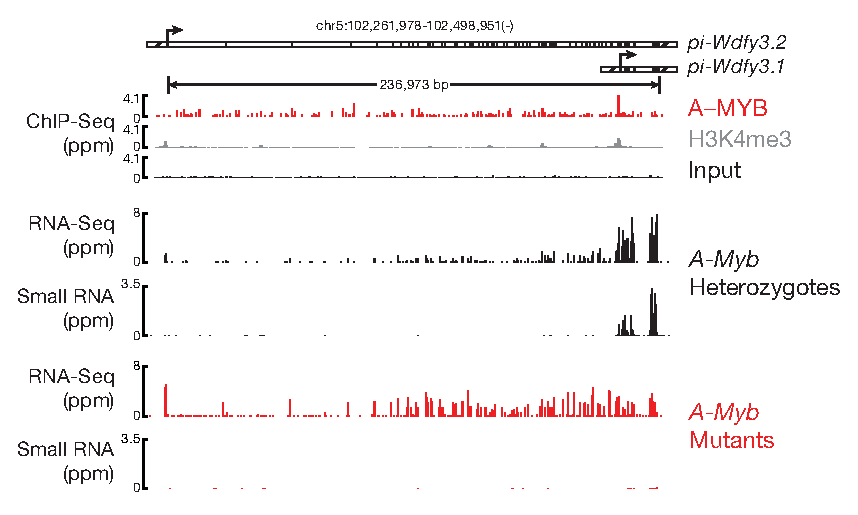
\includegraphics{Figures/Discussion/pi-wdfy3.eps}
      \caption[\wdfy{} locus expresses both mRNA and piRNA precursor form in testes]
      {\wdfy{} locus expresses both mRNA and piRNA precursor form in testes\\[0.25cm]
        The mouse genomic locus \wdfy{} expresses both a traditional mRNA form, originating from an upstream TSS, and a piRNA precursor transcript from a downstream TSS. The piRNA precursor form appears to originate from an A-MYB-bound promoter, and is expressed in \amyb{} heterozygous mice. Also small RNAs (piRNAs) mapping to this locus are only observed in \amyb{} heterozygous mice, and not in \amyb{} mutant mice.
        }
      \label{Disc:fig:wdfy3}
      \end{figure}

    These results indicate that A-MYB drives transcription of the shorter \textit{pi-Wdfy3.1} isoform, but not longer isoform, annotated elsewhere simply as \textit{Wdfy3}. A general phenomenon of piRNAs mapping to the 3\textprime~-UTR of mRNAs has been reported \citep{Robine2009}. How does a cell discriminate between these two transcripts

    Recently it was demonstrated that virtually all RNAs interact with the ribosome \citep{Ingolia2011}. This observation was later refined to state that only mRNAs display a strong ``Ribosome Release Score (RRS)'' indicative of read-frame engagement \citep{Guttman2013}. Therefore, it is not surprising that preliminary results support precursors being traversed by ribosomes (Xin Zhiguo Li, unpublished). Additional experiments and bioinformatic analysis may tease out sequence elements the assist in precursor discrimination from mRNAs by the ribosome, similar to the RRS for traditional ncRNAs.

    Beyond ribosome profiling, what are other potential experimental approaches that could be used to gain insight into the biology of mammalian piRNA precursors?

  \subsection{Precursor Interactions}
    \label{Disc:subsec:Labeling of precursors}

    While intergenic piRNA loci share many features with other Pol II transcript classes (Figure \ref{SeqZipMethod:fig:piRNA precusor Tx features}) one almost half contain no introns. Visual inspection using genome browsers and the HTS datasets described in Chapter \ref{MolCel} revealed how unique these loci are from the rest of the transcriptome.

    As discussed in sections \ref{Intro:subsec:Alternative Splicing} and \ref{Intro:subsec:Splicing Code}, splice sites and SRE are recognized amidst a sea of extremely similar ``crytic'' sequences. The spliceosome is remarkably efficient at determining the correct elements to use. Spliceosomal components assist in choosing from this the overwhelming set of sequences. \citet{Berg2012} identified the snRNP U1 as a key suppressor of cryptic polyadenylation site (PAS) use. This suppressor activity is in contrast to its primary role in the definition of 5\textprime~splice sites. Perhaps a similar mechanism is acting on cryptic splice sites contained within precursor transcripts. What experiments could be used to identify precursor interacting molecules, protein and RNA both?

    Coincident with HTS development, methodology to measure genome-wide interactions have also made considerable advances \citep{Konig2011}. Methodologies to capture \{Protein::RNA\} interactions include ``HTS-CLIP'' \citep{Licatalosi2008}, ``PAR-CLIP'' \citep{Hafner2010}, and ``iCLIP'' \citep{Konig2010}. \{DNA::RNA\} interactions are measurable using ``ChIRP'' \citep{Chu2012}, \{RNA::RNA\} interactions by ``RAP'' and ``CLASH'' \citep{Engreitz2013,Helwak2014}. These approaches could be applied to determining piRNA precursor transcript interacting molecules. However, there are some important caveats that warrant discussion.

    Techniques mentioned above that investigate \{Nucleic acid::Protein\} interactions require a target protein. This has already been done for MILI and MIWI in postnatal testes \citep{Vourekas2012}, and few additional interacting proteins are known, limiting the number of proteins to investigate. Obvious initial candidates include MitoPLD, Mvh \citep{Lasko2013} (the mouse homologue of Vasa) and numerous Tudor-related proteins \citep{Chen2011}.

    Genome-wide study of \{Nucleic Acid::Protein\} interactions typically require cross-linking \citep{Chodosh2001} using either ultra violet light or reagents such as glutathione. This requirement is why most original reports of these techniques are performed in cell culture (due to the relative easy of exposing the sample to the cross-linking reagent). Currently, the process of piRNA biogenesis has only been reproduced \textit{in vitro} using silk worm cell culture extracts \citep{Kawaoka2009,Kawaoka2011}, a system which is likely far from that of pachytene biogenesis and function in mice. Therefore, application of these techniques to mammalian piRNA pathway study would require testes sectioning prior to cross-linking. \citep{Vourekas2012} worked around this requirement by detunicated testes and creating a cell suspension in a petri dish which was then irradiated.

    Another potential work-around for would be to perform these studies in mature (or \textit{maturing}) sperm. Sperm develop and mature as they move through the seminiferous tubules and into the epididymis, where piRNAs are known to be ``sequence-able'' in humans \citep{Jones1999,Li2012a}. However, how much of exciting biology driven by piRNAs has already occurring once sperm have transitioned into the epididymis?

    \{Nucleic Acid::Nucleic acid\} interactions typically require a ligation step, the efficiency of which is typically very low \citep{Helwak2014}. Also, the ``ChIRP'' protocol is done in crude cell extract, where RNAse H is a concern when using DNA probes to pull down and query RNA. Given that precursor transcripts seem to be rapidly processed (section \ref{SeqZipMethod:sec:piRNA precursor by SeqZip}), these methods may require prior enrichment, perhaps using RNACapture \citep{Mercer2014}. Given recent developments into the CRISPR/CAS9 system for genome-editing \citep{Sander2014}, the ``CLASH'' approach to look at \{RNA::RNA\} interactions for precursor transcripts is attractive as the requirement for a tagged protein is no longer as large a barrier.

    There are many applications to piRNA biogenesis biology for these experimental techniques as they evolve and become more robust. Increased resolution of time points, proteins, and species examined will help to create a comprehensive purpose for piRNA in the maintenance of mammalian male fertility.

  \subsection{Precursor Location}
    \label{Disc:subsec:Imaging of precursors}

    A drawback of all the methods and approaches discussed above is that they do not maintain the anatomical and cellular location of transcripts. Localization of RNA has been important for decades \citep{Rebagliati1985}, and was recently shown in a large screen in \flies{} embryos to be the rule rather than the exception \citep{Lecuyer2007}.

    The most important question for mammalian \textit{pachytene} piRNAs is \textit{What are they doing}? We know that they are essential for the health of the species, as discussed in section \ref{MolCel:sec:Introduction}, and piRNA-pathway mutants are sterile. What could these small RNAs, with complementarity to nothing but themselves, be doing? 

    The cellular location of precursor piRNA transcript processing is not known. The most accepted hypothesis is that precursor transcripts are processed into mature piRNAs with machinery tethered to chromatoid bodies \citep{Meikar2011,Meikar2014} or another structure similar to Drosophila Nuage. Knowledge of \textit{where} where mature piRNAs are generated would provide clues into larger biogenesis mechanistic details.

    Identifying the location of mature piRNA processing from precursor transcripts could be achieved through development and application of techniques to visualize precursors in a dense sea of other RNA, including mature piRNAs. Improvements in \textit{in vitro} FISH experiments allow for discrimination of isoforms resulting from alternative splicing \citep{Lee2014}. Robust FISH-type experiments could be used to investigate cellular and anatomical locations of precursor transcript processing. The SeqZip methodology could even be used in this regard (see section \ref{Disc:subsubsec:SeqZip and Single-Molecule FISH}).

    Beyond FISH, direct imaging of precursor transcripts could be accomplish by engineering MS2 loop sequences into piRNA-generating genes similar to experiments performed in the the Singer lab \citep{Park2014}. This would be assisted by the previously mentioned CRISPR/CAS9 systems. Mice expressing precursors containing MS2 loops could be crossed with those containing MS2 Bacteriophage capsid protein fused to GFP (MCP-GFP). Using this system precursors could potentially be visualized in real time or at least in real locations.

  \subsection{Precursor Sequencing}
    \label{Disc:subsec:Sequencing of Precursors}

    Very recently methods demonstrating sequencing \textit{in situ} have been published \citep{Ke2013,Lee2014a}. These methods represent a major improvement over the single-cell sequencing approaches discussed in section \ref{Intro:subsec:Types of HTS}. Building upon the principles of FISH, \textit{in situ} sequencing allows for novel sequence discovery, multiplex investigation, and cellular location RNA. Could \textit{in situ} sequencing be used to learn more about piRNA precursor biology?

    FISSEQ, reported by \citet{Lee2014a}, uses rolling circle amplification to create a 3D grid of highly-concentrated DNA (``nanoballs''), originating from a single RNA/cDNA. SOLiD sequencing is used to determine 27--30 bases from each nanoball. Confocal microscopy is used to assign the sequence to 3D location within the sample. Read lengths for FISSEQ would make it difficult to distinguish mature piRNAs from precursors. An experimental scheme, perhaps exploiting the methylation of mature piRNAs, would be necessary to ensure sequencing of piRNA precursors or intermediates.

    Whether by determining the interacting molecules, physical location, or \textit{in situ} sequence, more advanced techniques are required to advance our understanding of this novel and exciting cellular process in a complex organ that perpetuates mammalian species.

\section{Future of RNA-templated DNA-DNA ligation}
  \label{Disc:sec:SeqZip Improvements}

  The SeqZip methodology as developed and described in Chapters \ref{SeqZipPaper} and \ref{SeqZipMethod} works adequately and robustly for characterization of relatively simple (\cd{}) to extremely complex (\dscam{}) genes. However, there is substantial room for optimization. The improvements, modifications, and applications discussed below support continued use of SeqZip in RNA research.

  \subsection{An Optimized SeqZip Examination of Coordinated Splicing}
    \label{Disc:subsec: Ideal SeqZip exp. to look for Coordination}

    If I could go back in time 4 years and still possess the knowledge and abilities that I do now, I would have approached a genome-wide study of coordination in splicing using SeqZip differently. I would have focused on alternative first exon use and potential coordination with downstream cassette exons. I would have mined newly-generated RNA-Seq data \citep{Wang2008, Pan2008} to limit identified targets for sufficient variation and expression. 

    Following target identification, I would have automated the ligamer design process (see Appendix \ref{Appendix:AutoMatedLigamerAssembly}), to create a database of the required ligamers. At least three ligamers would be required per event, with very little duplicated use of ligamers. The number of ligamers required would preclude the use of standard synthesis (even in a 384-well plate format). Therefore, I would have pursued printing the ligamers on a custom microarray, similar to products offered by \href{http://www.nimblegen.com/}{Nimblogen}. These ligamers would be barcoded and priming sequences included such that short (50nt) paired-end reads could reliably identify the templated first and cassette exons. 

    Using this complex ligamer pool, I would have further optimized the SeqZip assay, including a barcoding scheme to quantify the number of ligation events per \{alt first exon::cassette exon\} pair. Also, libraries would have been amplified using a digital PCR scheme. This would allow determination of PCR jackpots and enhance read quantification \citep{Shiroguchi2012a}. Finally, the data would be aligned against a reference of all \{alt first exon::cassette exon\} pairs and any potential coordination determined.

    If I could have done the experiment described above, I feel the full potential and utility of the SeqZip method could have been realized and generated new and valuable knowledge for the field of gene expression.

  \subsection{LNA-containing ligamers and T39A Rnl2}
    \label{Disc:subsec:LNA-Containing ligamers and T39A Rnk2}

    The use of an RNA-base on the 5\textprime~side of the nick encourages a C3\textprime~\textit{endo} sugar pucker for the base, placing the 3\textprime~OH in an apical orientation relative to the the AMP leaving group (Figure \ref{Disc:fig:Rnl2 and suger pucker}) \citep{Nandakumar2006}. With lowered costs of oligo synthesis, incorporation of 2\textprime~OMe at the penultimate and ultimate bases of the 5\textprime~nick ligamers should greatly increase ligation efficiency, as these are the primary substrate-specificity determinants of Rnl2 due to this conformational constraint \citep{Nandakumar2004a, Nandakumar2006}.

    \begin{figure} % Rnl2 Suger Pucker
      \centering 
      \includegraphics{Figures/Discussion/Rnl2_and_suger_pucker.eps}
      \caption[Sugar pucker in Rnl2 structures]
      {Sugar pucker in Rnl2 structures \\[0.25cm]
        Using two different nucleic acid substrate combinations crystallized with Rnl2, \citet{Nandakumar2006} demonstrates the effect of 3\textprime~and 2\textprime~ identify of the base at the 5\textprime~side of the nick: Left) The crystal structure (PDB: 2HVS), containing a 2\textprime~ position deoxy residue, displays a DNA-like C2\textprime~\textit{endo} sugar pucker. In contrast to Right) where the crystal structure (2HVR) contains a 2\textprime~ hydroxyl and displays an RNA-like C3\textprime~\textit{endo} sugar pucker.
        }
        \label{Disc:fig:Rnl2 and suger pucker}
        \end{figure}

    \citet{Nandakumar2004a} demonstrated the importance of the ribose at this penultimate position, evidenced by a 50-fold reduction in turnover for substrates containing a 2\textprime~H substitutions. Figure \ref{Disc:fig:Rnl2 and suger pucker} shows that Threonine 39 (T39) hydrogen bonds with both the 2\textprime~OMe and 3\textprime~O of the penultimate sugar. A T39A mutation did not phenocopy the 2\textprime~H substitution on the penultimate sugar, indicating that the structural constraint of sugar pucker is important for efficient ligation. These results support the use of a T39A Rnl2 mutant for increased RNA-templated DNA-DNA ligation efficiency, as the mutant would have one less molecular requirement for an RNA substrate.

    Future versions of the SeqZip assay could use a combination of LNA modified bases \citep{You2006} at either the penultimate or terminal residues (or both) on the 5\textprime~side of the nick in order to increase specificity and efficiency. The combination of modified ligamers and the T39A Rnl2 mutant could enhance the efficiency of RNA-templated DNA-DNA ligations required by SeqZip.

  \subsection{Thermostable Ligases}
    \label{Disc:subsec:Thermostable Ligases}

    The use of LNA-containing brings up issues involving off-target hybridization. Directed protein evolution of Rnl2 \citep{Stemmer1994, Romero2009a} could be used to develop a thermostable variant of the enzyme, similar to variations of DNA ligase that have been used for years \citep{Barany1991}. Use of LNAs and elevated ligation temperatures could alleviate off-target hybridization events reducing both nonproductive hybridization and non-templated ligation. This would also allow for use of reduced overall ligamer concentrations, in line with the optimal SeqZip experiment described in section \ref{Disc:subsec: Ideal SeqZip exp. to look for Coordination} and ligamer synthesis on microarrays.

  \subsection{Other SeqZip Applications}
    \label{Disc:subsec:Future Uses of SeqZip}

    SeqZip can be used in many different forms of RNA sequence characterization. An incomplete illustration of these applications is shown in Figure \ref{Disc:fig: Panel of SeqZip Applications}. Three novel applications are discussed below:

    \begin{figure} % SeqZip uses Panel
      \centering 
      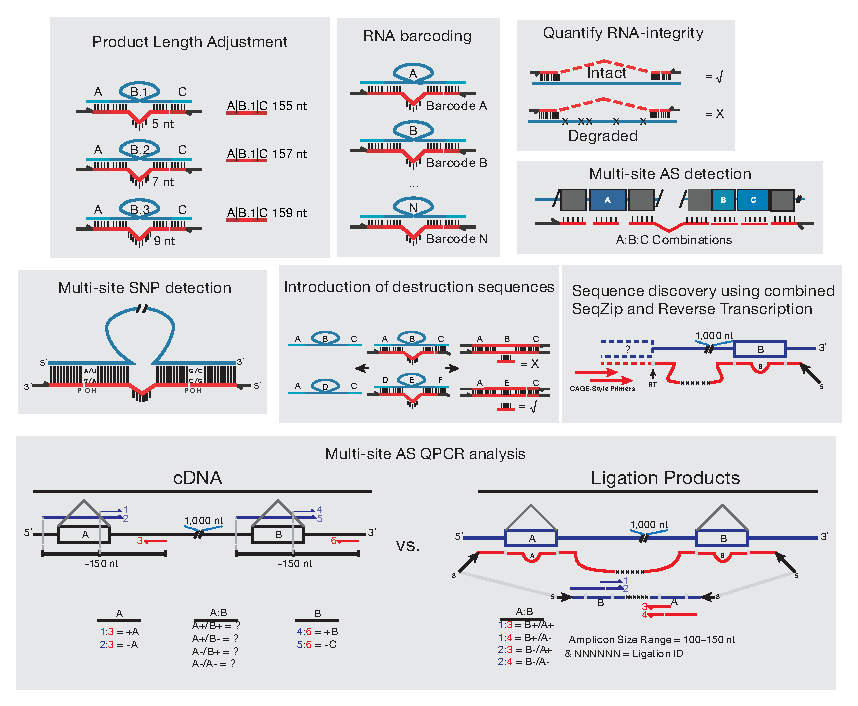
\includegraphics{Figures/Discussion/SeqZipUses.eps}
      \caption[Proposed uses of the SeqZip methodology]
      {Proposed uses of the SeqZip methodology \\[0.25cm]
        Shown are general applications of the SeqZip method to profiling RNA sequences. Top row examples are substantiated by experiments described on Chapters \ref{SeqZipPaper} and \ref{SeqZipMethod}.  Middle and bottom rows are hypothetical, but logical, extensions of the method.
        }
      \label{Disc:fig: Panel of SeqZip Applications}
      \end{figure}

    \subsubsection{Multi-site SNP detection}
      \label{Disc:subsubsec: Multi-site SNP Detection}

      The concept of connectivity in sequence can be applied not only to exons, or long stretches of RNA, but even to single-nucleotide polymorphisms (SNPs). SeqZip could be used to profile potential SNPs contained within the same transcript and therefore within the same allele (Figure \ref{Disc:fig: Panel of SeqZip Applications}). For maximal benefit and specificity, care should be taken as to where the variant ligamers bases are placed respective to the 5\textprime~ or 3\textprime~ side of the ligation site. For example, \citet{Chauleau2013b} have demonstrated the importance of proper base pairing at the 3\textprime~OH side of the nick.

    \subsubsection{SeqZip and single-molecule multi-site FISH}
      \label{Disc:subsubsec:SeqZip and Single-Molecule FISH}

      \begin{figure} % Multi-site Fish using SeqZip
        \centering 
        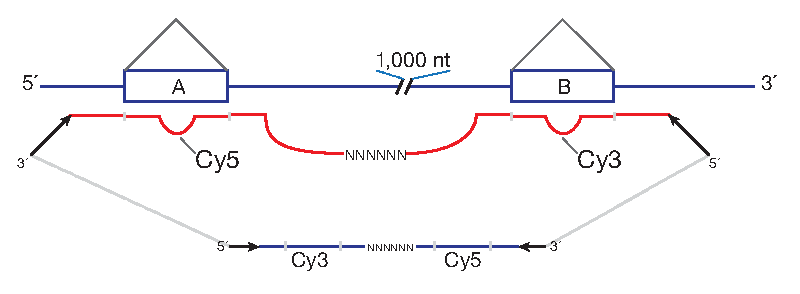
\includegraphics{Figures/Discussion/MultiSiteFish.eps}
        \caption[Multi-Site smFISH using flourophore-containing ligamers]
        {
          Multi-Site smFISH using flourophore-containing ligamers
          \\ [0.25cm]
          The simplest form of a multi-site FISH SeqZip experiment. Five ligamers are used, with two hybridizing to the beginning and end of a target RNA sequence (e.g. and exon), and having unique fluorescent labels (Cy3 and Cy5 in this case). The use of the third ligamer, containing an addressable barcode is used to report on these two ligamers hybridizing to the same RNA. Use of flanking ligamers allows for amplification, downstream analysis, and trouble shooting.
          }
        \label{Disc:fig:MultiSite FISH using SeqZip}
        \end{figure}

      A logical extension of the multi-site SNP detection application described above is the use of SeqZip in multi-site FISH probes Figure (\ref{Disc:fig:MultiSite FISH using SeqZip}). Advances in FISH, microscopy, fluorescent moieties, and image processing are making this type of experiment more approachable. A multi-site FISH SeqZip experiment could be used to ask some of the questions described in section \ref{Disc:subsec:Imaging of precursors}, including precursor integrity and location, without the need for downstream processing.

    \subsubsection{Introduction of destruction sequences}
      \label{Disc:subsubsec:Intro of Desctruction Sequences}

      Introduction of unique sequences into a ligation product is a powerful feature of SeqZip. In addition to the other proposed uses (barcoding, sites of priming, sequence diversity, etc) the sequences introduced could also be used to \textit{eliminate} ligation products. Restriction enzymes or elimination via selective hybridization, similar removal of ribosomal RNA sequences during HTS library preparation \citep{Chen2011a}, are two potential ways to remove products of ligation.

    \subsubsection{Re-purposing the SOLiD Platform}
      \label{Disc:subsubsec:SOLiD Platform for SeqZip}

      Custom sequences within ligamers could also be used to generalize exon identity. Put another way, ligamers representing the first exon of a message could be given a specific barcode, second exons another barcode, and so on. Then, using a sequencing platform such as SOLiD and custom hybridization/sequencing oligos, florescent signal would report not the sequence, but the numeric ID of the exon within the target message. A few rounds of traditional sequencing could identify the mRNA from each spot, and a simplistic schema of exon arrangement could be interpreted from the ligation product. This would require major SeqZip optimization, bioinformatic transformation of a given transcriptome annotation, transcriptome-wide design and synthesis of ligamers, and customization of the SOLiD ligation chemistry. But it would be extremely useful and informative for complete and routine transcriptome quantification.

\section{Final Thoughts}
  \label{Disc:sec:Final Thoughts}

  This thesis has introduced the complexity, purpose, potential, and challenges of transcriptome study. There is no comparison between these issues with that of the DNA genome. The next period of biomedical knowledge will be heralded by advances in transcriptome analysis. This section discusses how scientists need to grow with technology.

  \subsection{Science vs. Engineering}
    \label{Disc:subsec:Science and Engineering}

    \begin{quote}
      \itshape 
      \singlespacing
      ``There is a general attitude among the scientific community that science is superior to engineering.'' --- \citep{Macilwain2010}

      ``Science is about what is; engineering is about what can be. Engineers are dedicated to solving problems and creating new, useful, and efficient things.'' --- Neil Armstrong
      \end{quote}

    A common schism between technically-oriented individuals is whether or not they identify themselves as an engineer or a scientist. The first quote, from an article published in \textit{Nature}, communicates a clear bias in academic circles of the importance of the \textit{why} over the \textit{how}. In essence, how one prioritizes these questions categorizes individuals as scientists (why is important) or engineers (how is more important). The second quote, from the first man to walk on the Moon, Neil Armstrong, highlights what motivates a self described ``engineer'' and ``geek.'' How does a graduate system---training PhDs for careers in life science---educate individuals who fall into these two fundamentally different belief systems?

    When searching for a lab I told professors that I wanted to work on a technology development project. A typical response was, ``That's not what we do here.'' As someone who is more interested in the ``how'' over the ``why,'' this began a brief period when I thought I had made the wrong choice leaving industry and going back to graduate school. What was the basis for this aversion to technology development? The same article in \textit{Nature} states that this feeling toward engineering may be attributed\ldots

    \begin{quote} 
      \itshape 
      \singlespacing
      \ldots partly to a ``linear'' model of innovation, which holds that scientific discovery leads to technology, which in turn leads to human betterment. This model is as firmly entrenched in policy-makers' minds as it is intellectually discredited. As any engineer will tell you, innovations, such as aviation and the steam engine, commonly precede scientific understanding of how things work.
      \end{quote} 

    In fact, some of the most notable breakthrough scientific discoveries, including many made by Nobel Laureates, demonstrate a clear integration of both the scientific method and practical application. For example, the 2007 award in Physiology and Medicine was given for ``discoveries of principles for introducing specific gene modifications in mice by the use of embryonic stem cells.'' By combining principle discoveries an indispensable technique in modern genetics was created---gene targeting. The feeling of which is more important, the principle discoveries or the application thereof, is likely what separates a scientist from an engineer.

    The importance of technology to the advancement of science in general is not limited to anecdotes resulting in a Nobel prize. A quick scan of the most \href{http://www.pnas.org/reports/most-cited}{highly-cited} papers in the \textit{PNAS} reveals that the top 13, indeed \textit{all} 13, describe a novel methodology or technique. Sequencing of DNA, microarray analysis, tetracycline-inducible promoters, recombinant adenovirus, and site-specific mutagenesis are just a handful of the tools on the list. This effect can also be seen in \href{http://simplystatistics.org/2014/04/07/writing-good-software-can-have-more-impact-than-publishing-in-high-impact-journals-for-genomic-statisticians/}{computation biology}, where transformative algorithms, such as BLAT \citep{Altschul1990} and Bowtie \citep{Langmead2009} attain citations well beyond a typical paper in their journal of publication, indeed far more than most primary research articles.

    The growth of big datasets is forcing all in biomedical research to think like an Engineer. At least two major concerns require immediate attention: How to store the data and how to analyze it?

  \subsection{The Data Deluge}
    \label{Disc:subsec:Dealing with Data Deluge}

    \begin{quote}
      \itshape
      \singlespacing
      ``The HiSeq X Ten is sold as a set of 10 or more ultra-high throughput sequencing systems, each generating up to 1.8 terabases (Tb) of sequencing data in less than three days or up to 600 gigabases (Gb) per day, per system, providing the throughput to sequence tens of thousands of high-quality, high-coverage genomes per year.'' \\
      \indent ---\href{http://bit.ly/PZpegZ}{Illumina Press Release}
      \end{quote}

    In a world where the HiSeq X, described above is a reality, biomedical researchers need to change how they approach every aspect of data analysis including storage, processing, and visualization. Evidence is mounting that replicates, not depth, are essential in differential gene expression \citep{Liu2014}. Replicates compound problems of keeping similar data and file types separate and tracked.

    How do we work with all this data? Systems need to be in place to track the necessary sample meta-data, analysis and modifications performed. Systems should aid in eventual public posting and sharing of HTS data. Laboratory information management systems (LIMs) and Electronic lab notebooks (ELNs) must be implemented in academic labs participating in copious amounts of HTS data generation and analysis.

    Once these systems are in place, the ability to navigate, via genome browsers \citep{Zweig2008,Robinson2011}, will be of critical importance to allow other members of the lab to reuse valuable datasets. Recent changes to the way aligned genomic data is stored and added to UCSC genome browsers is a good example of needed process improvements \citep{Raney2013}. Finally, efforts such as the Galaxy project will define how most academic labs perform future ``routine'' HTS analysis \citep{Blankenberg2010}.

  \subsection{Biologists need Computation Biological Skills}
    \label{Disc:subsec:Biologists need Comp Skills}

    Just 10 years ago, graduate students and PhDs in the fields of Molecular Biology or Biochemistry need not venture far from Excel or perhaps a statistical program with an advanced graphical interface (e.g. Prism or Graphpad). Software knowledge that stops at these tools and the rest of the Microsoft Office suite is no longer enough to generate big strides in Biomedical research.

    Working with tens of even hundreds of lines of data within a spreadsheet is manageable. Computers from 20 years ago had more then enough computing power to process these type of data. Data generated from most cutting edge projects can no longer be analyzed in a spreadsheet program. Many students and post-docs find that they are unable to analyze the data generated from months or years of tireless bench work. Faced with learning what is effectively a collection of new languages and awash in a sea of acronyms (e.g. LINUX, BASH, GNU, PERL, R) they reach out for help from a ``bioinformatics person.'' Perhaps the relationship and interaction with this personal is productive, leading to a collaboration and exciting new knowledge. Sometimes it isn't and the bench scientist shifts into one of three modes: wait, find another bioinformatic-minded collaborator; or collect more data.

    \begin{table} % Changes at the computer for Molecular biogists
      \caption[Changing computational tools for Molecular Biologists] 
        {
         Changing computational tools for Molecular Biologists
         }
       \label{Disc:tab:Comp tools for Molecular Biology}
       \footnotesize
\begin{tabular}{p{6cm}|p{8cm}}

\textbf{What is Used}            & \textbf{What Should be Used}                \\ \hline 
Word                             & Plain Text                                  \\ \hline 
Hand-inserted Citations          & Citation-management Software (e.g. Papers ) \\ \hline 
Paper Notebooks                  & Evernote or Commercial ELNs                 \\ \hline 
Excel for Storage                & Relational Databases (i.e. MySQL)           \\ \hline 
Excel for Analysis               & R                                           \\ \hline 
Local Code development \& backup & Online Code development (GitHub)            \\ \hline 
\end{tabular}



       \end{table}

    The ``wait'' mode is the most damaging, as it delays the progress of one's work and the advancement of science in general. Personally, I did not want to fall into this mode. Once the multiplex study described in section \ref{SeqZipMethod:sec:Multiplex Gene Study} reached a point where I had millions of sequencing reads but I could not find anyone to help me analyze the data, I decided to educate myself on the basic principles of Linux, the command line, and analysis of HTS data.

    A biologically-train individual who posses the knowledge of analysis of HTS datasets is an extremely powerful and empowering situation. This was recently communicated in \citet{Plocik2013}:

    \begin{quote} % Polick2013 Quote about insight without a Pipette
      \itshape 
      ``Such exercises will empower students to explore and assess the quantitative data published in the manuscripts that they read, which can no longer be assessed at a glance like the qualitative gel-based results on which molecular biology was founded. Ultimately, it will be equally important to know how to write code as it is to pipette.'' --- \citep{Plocik2013}
      \singlespacing
      \end{quote}

    The fact is that no one will care about a project as much as the student or post-doc who generated the data. Learning and training of computational skills bent on analyzing large datasets (see Table \ref{Disc:tab:Comp tools for Molecular Biology})should be central to the education in Biomedical sciences in the future.

\cleardoublepage